\documentclass[UTF8]{ctexart}
\usepackage{amsfonts}
\usepackage{amssymb}
\usepackage{graphicx}
\usepackage[]{algorithm2e}

\title{模式识别大作业 报告}
\author{黄豪硕 2014011??? \\ 苏克 2014011402}

\begin{document}
	
\maketitle

\section{问题介绍}

介绍一下题目。可以给出数据的截图来说明噪声的事情。【求补充】

\section{算法介绍}

为了完成数字分类的任务,我们打算采用的方法有:

\begin{itemize}
	\item 支持向量机(SVM):SVM可以用线性或非线性的核函数将输入空间映射至目标空间,通过在目标空间上划分超平面(决策平面)来进行分类。
	
	\item 多层神经网络(MLP):多层神经网络是一种解决高度非线性问题的模型,可以通过训练集优化参数,拟合出一个分类函数。由于多层神经网络的基本结构来源于人脑中的感知器,因此多层全连接结构的神经网络往往被称为“多层感知器(Multiple Layers Perception)”。
	
	\item 卷积神经网络(CNN):卷积神经网络是多层神经网络的“简化”,因为它使用同样的卷积核函数在输入向亮上通过往复卷积,将得到的结果通过一个激活函数(sigmoid或者relu),得到输出向量。对于图片分类的问题来说,CNN取得了广泛的成功。
	
	\item 限制玻尔兹曼机(RBM):【我不会~~ 求补充~~ 可以多写点】
\end{itemize}

\section{算法实现}

我们实现了以上几种算法,并且进行了简单的调参处理。我们使用原始的训练集对上述各个模型进行训练,之后令训练好的模型对测试集的输入数据给出自己的预测结果,并与测试集的标注结果相对比,求出模型在训练集上的预测准确率(以下简称准确率)。

我们保证以下结果的真实性:有些代码或许已经被注释掉,但是用户修改少量的代码就可以复现我们在这里给出的结果。如果对结果有任何疑问或质疑,欢迎邮件联系我们解决。

\subsection{SVM}

给出SVM的结果【求补充】

\subsection{MLP}

只要单层全连接结构(由1024维的输入直接连到10维)的MLP就可以迅速地训练出预测准确率达到100\%的模型。训练的几个关键参数如下:

\begin{itemize}
	\item learning rate: 0.001
	
	表示参数变化的速度(更具体地说,表示每一步迭代的过程中参数的变化)。
	
	\item weight decay:	1e-6
	
	表示较大的参数会带来多大的penalty。这个参数通常用于防止参数变得过大而过拟合。
	
	\item max epoches: 50
	
	表示总共进行50轮迭代。在每一轮迭代中,每个输入数据会且仅会被使用一次。
\end{itemize}

loss函数为categorical\_crossentropy(数字的label已经转换成one-hot形式),最后输出结果的分类器为softmax层。图\ref{MLP}表示了一次完整训练过程中,测试集上分类准确率与epoch的关系图。可以看到,在30个epoch过后,模型在测试集上的准确率就已经十分接近100\%。在50个epoch的训练过程结束之后,模型在测试集上的分类准确率达到了100\%。

\begin{figure}
	\centering
	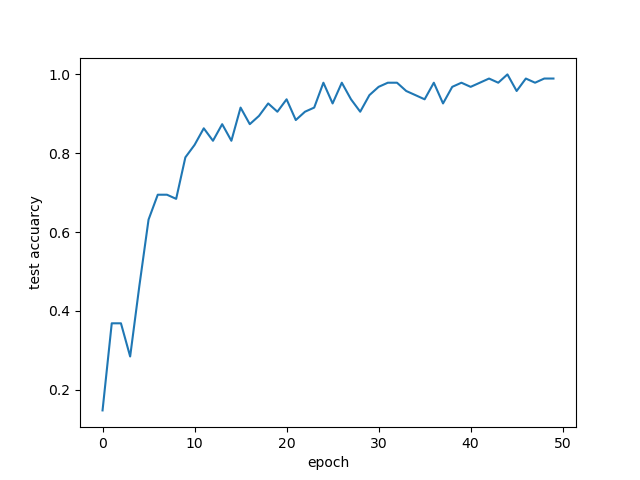
\includegraphics{nn}
	\caption{MLP 训练过程}
	\label{MLP}
\end{figure}

\subsection{CNN}

通过较为复杂的CNN网络,可以在非常少的epoch之内就训练出效果足够好的模型。我们所建立的CNN模型如图\ref{cnn_model}所示。输入的图片经过两次卷积层之后,通过MaxPooling层进行采样,其结果被看作是一维向量,又经过全连接层才输出分类的结果。除最后一层输出分类结果采用softmax激活函数之外,其他激活函数均采用ReLU。

\begin{figure}
	\centering
	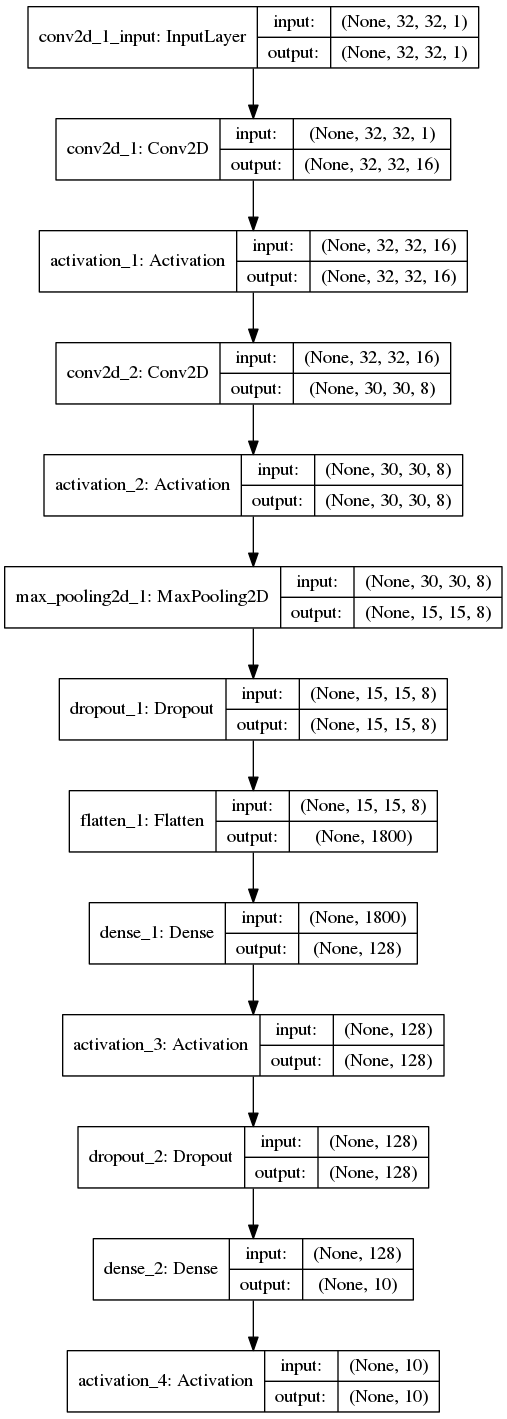
\includegraphics[scale=0.4]{model}
	\caption{CNN 结构}
	\label{cnn_model}
\end{figure}

训练该CNN的参数与上面训练MLP的参数相同。唯一的不同是,由于此模型训练更快,因此只需要20个epoch即可以得到100\%测试准确率的模型。整个训练过程中,测试准确率的变化如图\ref{cnn}所示。可以看到,在13个epoch之后,模型便可以达到100\%的准确率。

\begin{figure}
	\centering
	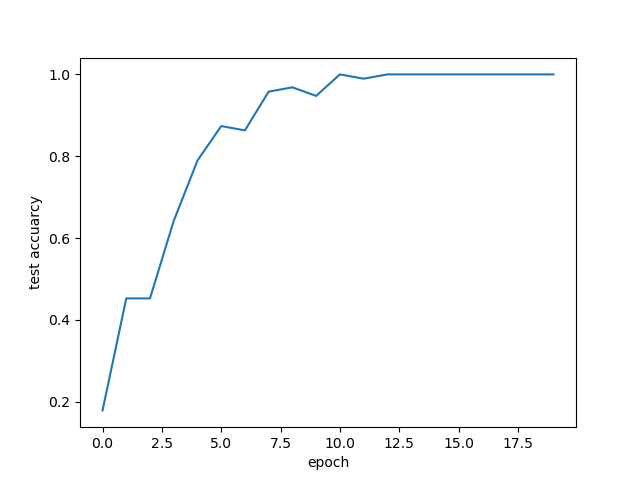
\includegraphics{cnn}
	\caption{CNN 训练过程}
	\label{cnn}
\end{figure}

\subsection{RBM}

给出RBM在1024维下的结果。【求补充】

\section{算法拓展:RBM维度压缩}

【求再吹点逼】

以上是朴素算法可以取得的优秀结果。我们并不满足于这些结果,希望可以进行一些拓展研究。我们主要关注RBM模型。RBM模型的表达能力和隐层向量的长度有很大的关系:如果隐层向量够长,训练RBM几乎一定可以得到足够优秀的结果。但是如果将RBM隐层

【给出降到64维的准确率结果(给出一个图表,画出维度减少对RBM性能的影响)】

对于隐层向量长度仅为64的RBM来说,其表达能力已经不足以解决本问题。我们希望通过一些自动的预处理方法对训练集(甚至测试集)进行处理,使得64维的RBM也可以训练出足够优秀的准确率。

\subsection{基于图形像素先验概率的噪声处理}

我们首先考虑降噪处理。传统降噪方法在这个问题上或许不甚可行:对于噪声比较大的输入数据来说,噪声和数字本身已经难以分辨。图\ref{train_set_sample}给出了一个训练集中的例子,可见噪声的“频率”和数字已经别无二致。

\begin{figure}
	\centering
	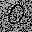
\includegraphics{train_set_sample}
	\caption{训练集一例}
	\label{train_set_sample}
\end{figure}

因此,我考虑采用更符合题目性质的降噪方式。因为训练集中仍然有很多没有噪声,或者噪声不太明显的数据,因此我们可以考虑通过计算每种数字的图形上每个像素上颜色值的期望来判断一个位置上的颜色有多大的可能性为噪声。这是一句比较绕的话,我们接下来会给出其形式化的定义。

考虑训练集$\{(I_n, L_n)\}$。其中,$I_n$表示第n张32*32大小的图片,每个像素值为0到1的浮点数,即$0 \leq I_n(i, j) \leq 1$。像素值为1代表白色。为了数学上的方便,我们将数据集的黑白进行了颠倒,即将原来白底黑字的图片改为了黑底白字。这样,“字”,或者说“图案”的部分的像素值比“背景”的部分像素值要大。数据集中$L_n$表示第n张图片对应的数字,为0到9的整数。

“降噪”的本质就是对于每个使得$I_n(i, j)$非零的位置$(i, j)$,判断这个“点”是数字的一部分还是噪声的一部分。具体的做法如下:

通过训练集,我们可以计算出某个数字$k$的图片上,$(i, j)$位置上的像素值是数字的概率$P_k(i, j)$:

$$ P_k(i, j) \propto \sum_{L_n = k}{I_n(i, j)} $$

它的物理含义是:对于一个数字k,我们找出训练集中所有该数字的图片,将其叠加起来。可以想象,图片与图片之间的数字部分大同小异,而噪声部分却各不相同。因此叠加之后,数字k的大致形状会显露出来;而噪声的部分则相对暗淡。在实际使用时,我们还进行了滤波处理,将正则化(normalize)之后的$P_k$矩阵中小于0.001的值滤成0,并进行第二次正则化。

在训练集上统计得到的10个数字的概率矩阵$P_k$分别如图\ref{prior}所示。我们把这些矩阵称为“图形像素先验概率矩阵”,因为这其中蕴含的是我们根据训练集统计得出的“先验信息”,与训练集无关。从图中可以看到,图形像素先验概率在图像中心,也就是对应数字的“数字”部分有比较大的数值;而在图像边缘的“噪声”部分则数值较小。


\begin{figure}
	\centering
	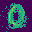
\includegraphics{0}
	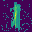
\includegraphics{1}
	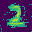
\includegraphics{2}
	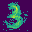
\includegraphics{3}
	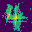
\includegraphics{4}
	
	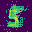
\includegraphics{5}
	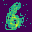
\includegraphics{6}
	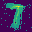
\includegraphics{7}
	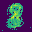
\includegraphics{8}
	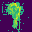
\includegraphics{9}
	\caption{图形像素先验概率矩阵}
	\label{prior}
\end{figure}

有了这些先验信息,就可以对训练集中的图像进行降噪了:

$$I^*_n(i, j) = I_n(i, j) * P_{L_n}(i, j)$$

即,根据一个图片所标注的标签选取相应的先验概率矩阵,并用这个概率矩阵对进行element-wise的乘积,所得到的就是降噪后的图像。可以想象,图像中属于噪声的某位置即使有数值(即的确存在噪声),也会因为先验概率矩阵中相同位置的概率值很低(甚至为零)而被消除。相反地,图像中属于数字的某位置如果有数值,由于相同位置的概率值较高,则不会被消除。在训练集上进行降噪的可视化结果如图\ref{noise}所示。最左边的图像是训练集中的原始图像$I_nb$,中间是数字“0”的先验概率矩阵$P_k$,右边是降噪之后的图像$I^*_n$。可以看到绝大多数的噪声被消除或减弱,而残留的噪声则也更多地局限在该数字形状的范围内。


\begin{figure}
	\centering
	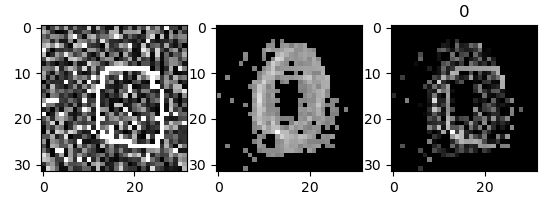
\includegraphics{noise}
	\caption{降噪结果}
	\label{noise}
\end{figure}


在对训练集进行降噪处理之后,由于测试集也包含了大量含有噪声的数据,两个数据集之间将会产生比较大的差异。因此,我们需要对测试集也进行类似的降噪处理。需要注意的是,我们不能使用测试集的标签信息,即我们只能采用unsupervised的方法进行降噪,而不能像训练集降噪这样根据数据的标签来选取最合理的先验概率矩阵。为了解决这一问题,我们可以用先验概率矩阵先做简单的预分类,然后用预分类的结果来选取合理的先验概率矩阵进行降噪。


预分类和测试集降噪的过程如下:

$$ L^*_m = argmax_{k}{\sum_{(i, j) \in \Omega}{P_k(i, j) * I(i, j)}} $$

$$ I^*_m(i, j) = I_m(i, j) * P_{L^*_m}(i, j) $$

这种降噪方法没有用到测试集的标签信息,只利用了训练集的统计信息。

经过降噪之后,64维RBM的测试准确率可以从67\%提升到89\%,这是一个可以接受的准确率。可见通过先验概率矩阵进行降噪之后,64维的RBM也具有了足够的表达能力,基本足够完成此问题的分类任务。


\subsection{另一个做法 ~~ 靠你了}

\subsection{RBM维度压缩实验结果}

\section{总结}

【靠你了!】


\end{document}